\section{Evaluation}
\label{sec:evaluation}

\begin{figure*}
	\centering
	\subfloat[Memcached --- 1 Process]{
		\label{fig:memcached_1p}
		%  \includegraphics[width=.32\textwidth,clip,trim = 18mm 213mm 117mm 20mm]{figs/eps/sim-rread-lat.eps}}
		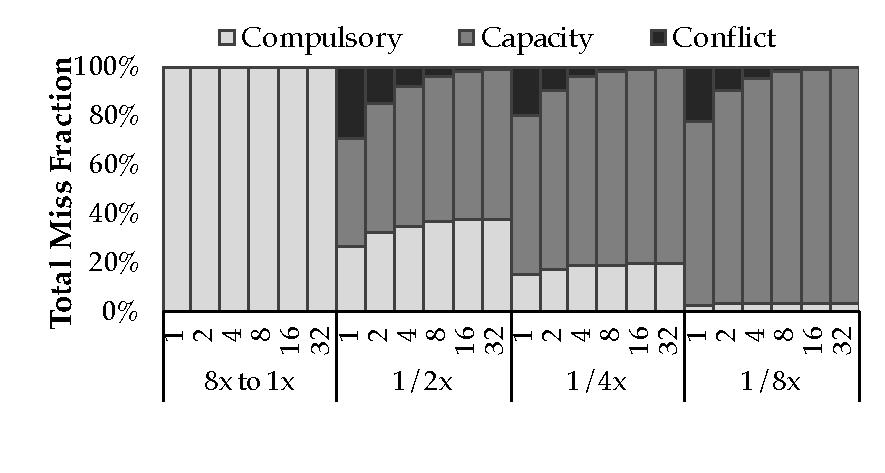
\includegraphics[width=.365\textwidth,clip]{graphs/memcached_assoc_1p-bw.pdf}}
	%  \hspace{.01in}
	\subfloat[RocksDB --- 1 Process]{
		\label{fig:rocksdb_1p}
		%  \includegraphics[width=.32\textwidth,clip,trim = 18mm 213mm 115mm 20mm]{figs/eps/sim-rread-bw.eps}}
		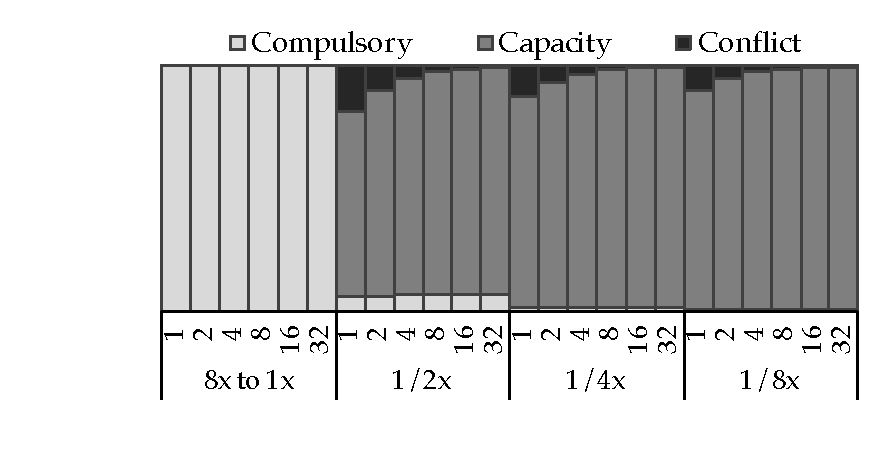
\includegraphics[width=.31\textwidth,clip]{graphs/rocksdb_assoc_1p-bw.pdf}}
	%   \hspace{.01in}
	\subfloat[Cassandra --- 1 Process]{
		\label{fig:cassandra_1p}
		%  \includegraphics[width=.32\textwidth,clip,trim = 28mm 217mm 115mm 20mm]{figs/eps/emu-rread-lat_cropped.eps}}
		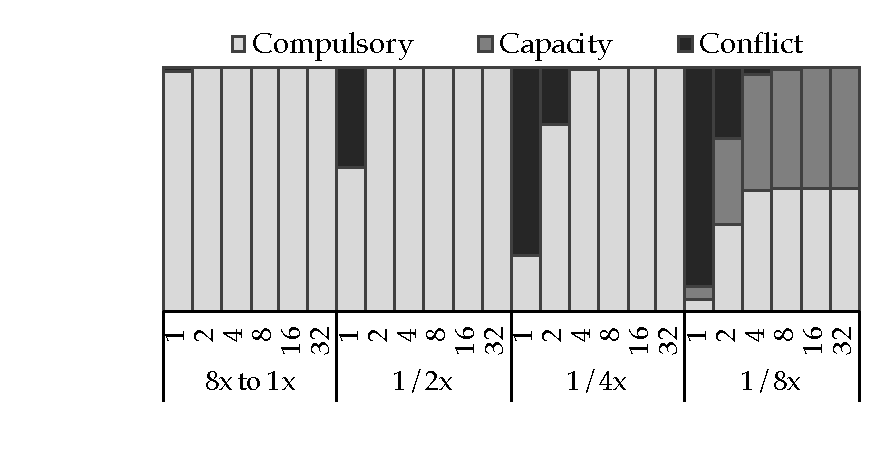
\includegraphics[width=.31\textwidth,clip]{graphs/cassandra_assoc_1p-bw.pdf}}
	\caption{Overall miss ratio broken down into compulsory, capacity, and conflict misses.
		\label{fig:miss_ratio}}
\end{figure*}

%%%%%%%%%%% Table: Methodology %%%%%%%%%%%
\begin{table}
	\begin{center}
		\caption{Workload description.}
		\scalebox{0.7}
		\small
		\vspace{0.01in}
		\label{table:workload}
		\renewcommand{\arraystretch}{1.0}
		{\scriptsize
			\begin{tabular}{ l  l }
				%\hline
				\toprule
				{\bf Workload}                  & {\bf Description}  \\
				%\hline
				%\hline
				\toprule
				\multirow{1}{*}{Cassandra}                       &  NoSQL data store running Yahoo's YCSB. \\
				%\hline
				\cmidrule{2-2}
				\multirow{1}{*}{Memcached}                      & Cache store running Twitter-like workload~\cite{lim:thin}. \\
				%\hline
				\cmidrule{2-2}
				%\multirow{2}{*}{Core Types}    & In-order (Cortex A8-like): 2-wide \\
				%		                               &  OoO (Xeon-like): 4-wide, 128-entry ROB \\
				%\hline
				\multirow{1}{*}{TPC-H}	& TPC-H on MonetDB column store (Q1-Q21). \\
				\cmidrule{2-2}
				\multirow{1}{*}{TPC-DS}	& TPC-DS on MonetDB column store (Queries of~\cite{kocberber:meet}). \\
				\cmidrule{2-2}
				%\multirow{2}{*}{L1-I/D Caches}	&	32KB, split, 2 ports, 64B blocks, 10 MSHRs, \\
				%							& 2-cycle load-to-use latency \\
				\multirow{1}{*}{MySQL} 			& SQL DBMS running Facebook's LinkBench~\cite{facebook:linkbench}. \\
				%\hline
				\cmidrule{2-2}
				\multirow{1}{*}{RocksDB}                             &  Store engine running Facebook benchmarks~\cite{facebook:rocksdb}. \\ %a canonical uniform request distribution. \\
				%\hline
				
				\bottomrule
				%\hline
			\end{tabular}
		} %small
	\end{center}
	\vspace{-0.1in}
\end{table}
%%%%%%%%%%% END Table: Methodology %%%%%%%%%%%%

\begin{figure*}[t]
	\centering
	\subfloat[Memcached --- 2 Processes]{
		\label{fig:memcached_2p_assoc}
		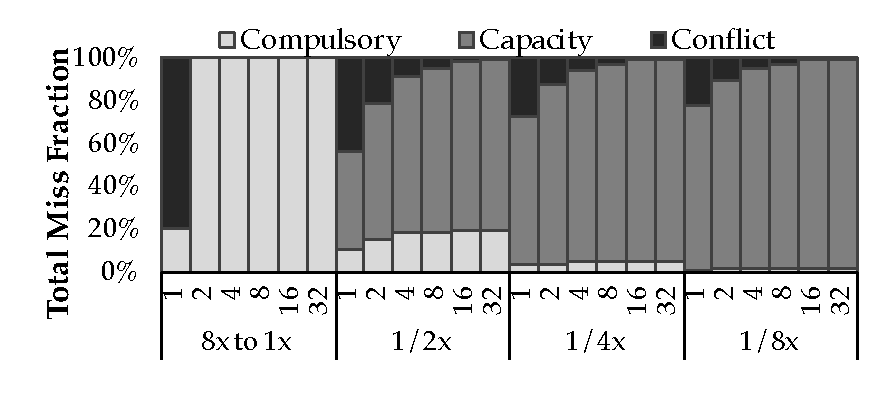
\includegraphics[width=.36\textwidth,clip]{graphs/memcached_assoc_2p-bw.pdf}}
	\subfloat[Memcached --- 4 Processes]{
		\label{fig:memcached_4p_assoc}
		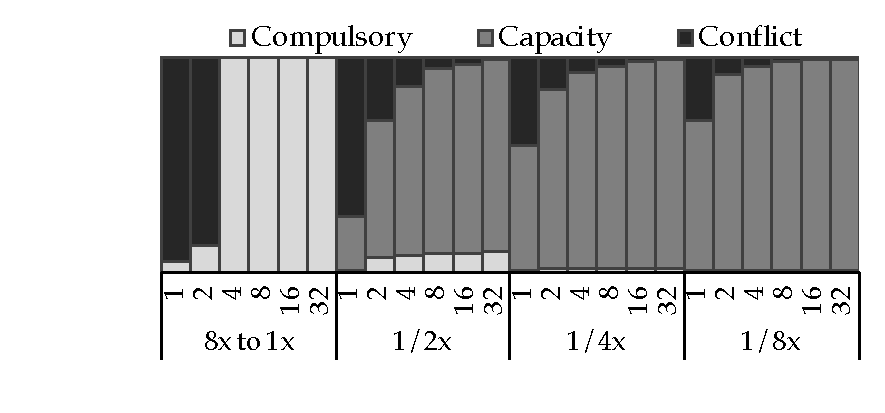
\includegraphics[width=.31\textwidth,clip]{graphs/memcached_assoc_4p-bw.pdf}}
	\subfloat[Memcached --- 8 Processes]{
		\label{fig:memcached_8p}
		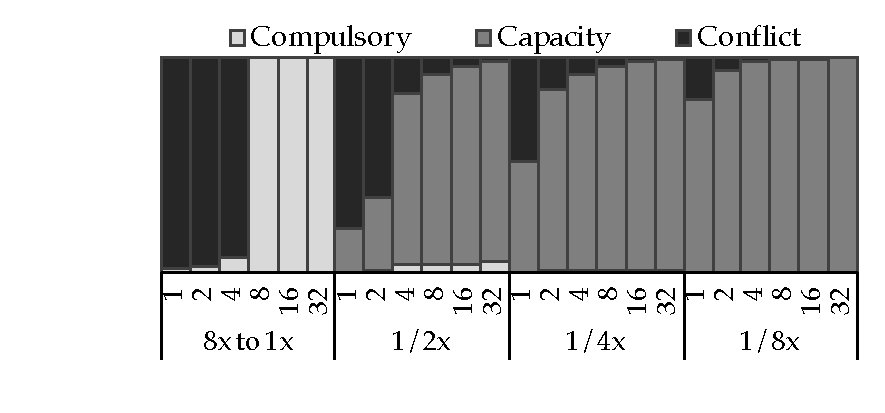
\includegraphics[width=.31\textwidth,clip]{graphs/memcached_assoc_8p-bw.pdf}}
	\hspace{.01in}
	\subfloat[RocksDB --- 2 Processes]{
		\label{fig:rocksdb_2p}
		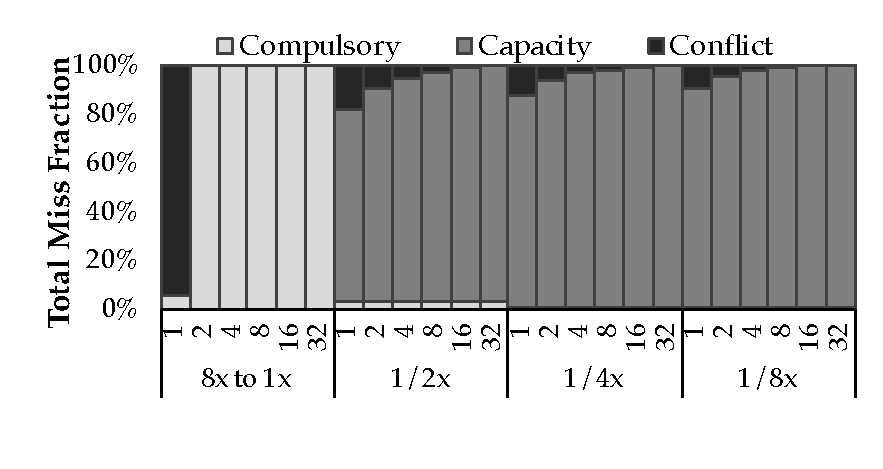
\includegraphics[width=.36\textwidth,clip]{graphs/rocksdb_assoc_2p-bw.pdf}}
	\subfloat[RocksDB --- 4 Processes]{
		\label{fig:rocksdb_4p}
		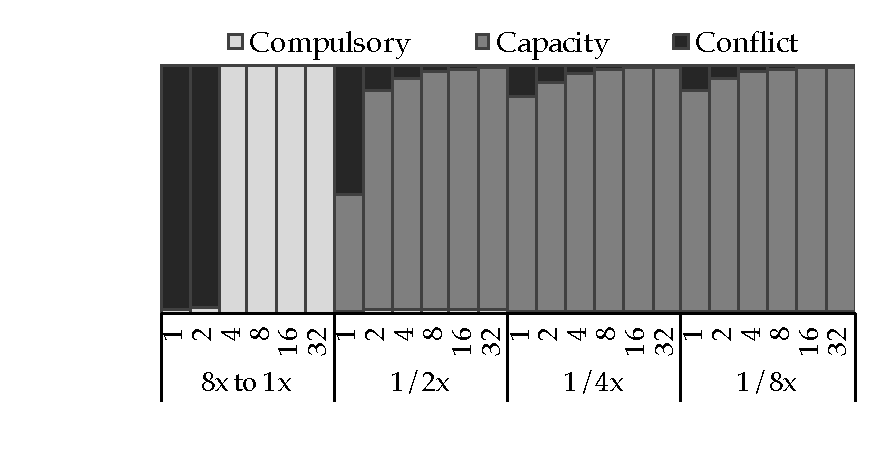
\includegraphics[width=.305\textwidth,clip]{graphs/rocksdb_assoc_4p-bw.pdf}}
	\subfloat[RocksDB --- 8 Processes]{
		\label{fig:rocksdb_8p}
		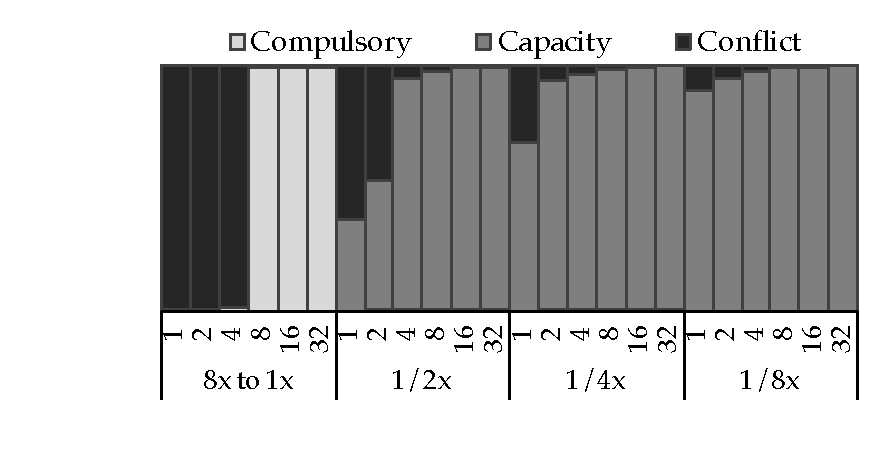
\includegraphics[width=.31\textwidth,clip]{graphs/rocksdb_assoc_8p-bw.pdf}}
	\hspace{.01in}
	\subfloat[Cassandra --- 2 Processes]{
		\label{fig:cassandra_2p}
		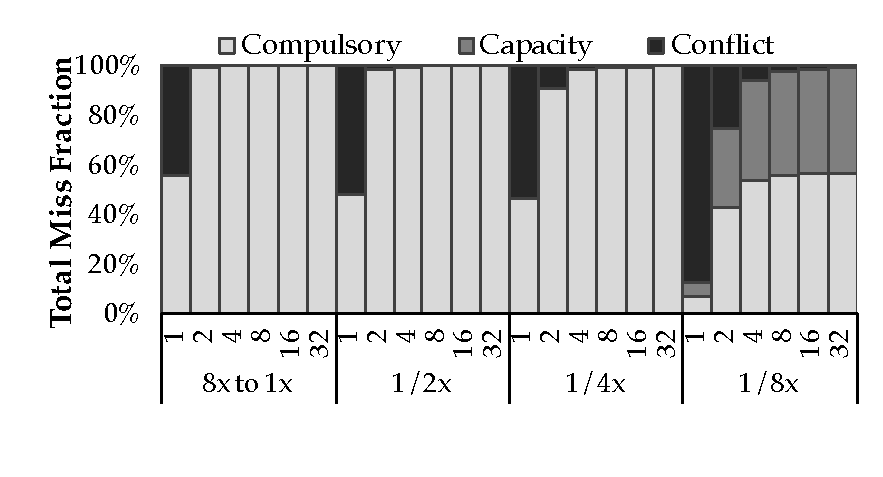
\includegraphics[width=.355\textwidth,clip]{graphs/cassandra_assoc_2p-bw.pdf}}
	\subfloat[Cassandra --- 4 Processes]{
		\label{fig:cassandra_4p}
		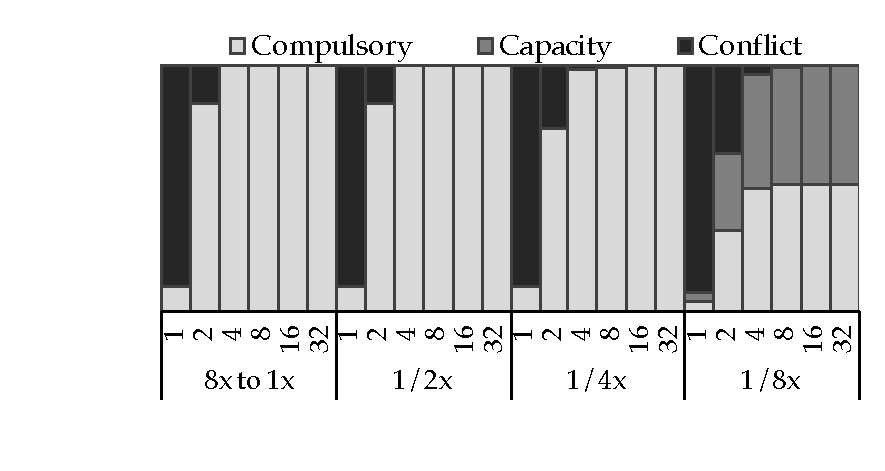
\includegraphics[width=.31\textwidth,clip]{graphs/cassandra_assoc_4p-bw.pdf}}
	\subfloat[Cassandra --- 8 Processes]{
		\label{fig:cassandra_8p}
		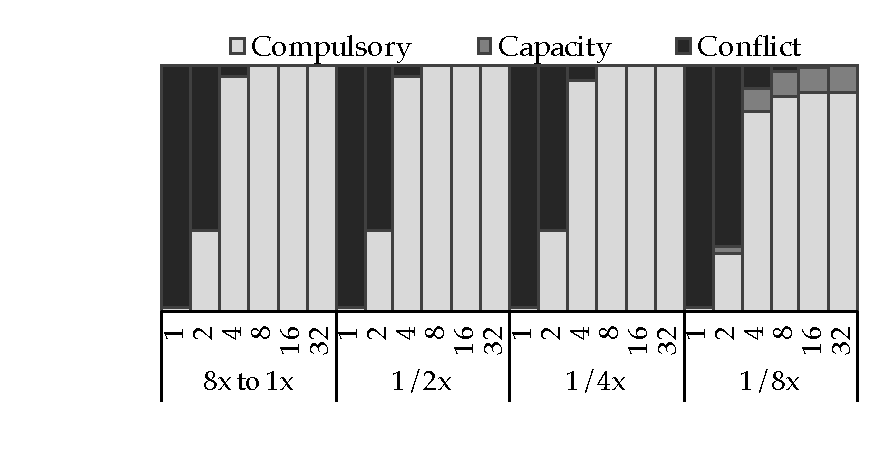
\includegraphics[width=.31\textwidth,clip]{graphs/cassandra_assoc_8p-bw.pdf}}
	
	
	\caption{Overall miss ratio broken down into compulsory, capacity, and conflict misses.
		\label{fig:miss_ratio_procs}}
\end{figure*}


%\javier{Points to come across:

%\begin{itemize}
%  \item Set-associativity doesn't increase page faults: 3C model %+ Memcached and RocksDB on real HW
%  \item TLB miss rate vs. working set for microkernels (hash %table, skip list, bst internal, bst external)
%  \item TLB miss penalty vs. working set (or sockets)
%  \item Fragmentation
%  \item $IPC =IPC_base + Penalty_tlb + Penalty_page_faults$
%\end{itemize}
%
%}


%\begin{figure*}[!h]
%\centering
% 
%  \subfloat[In-memory scenario.]{
%  \label{fig:speedup_memory_in}
%
%   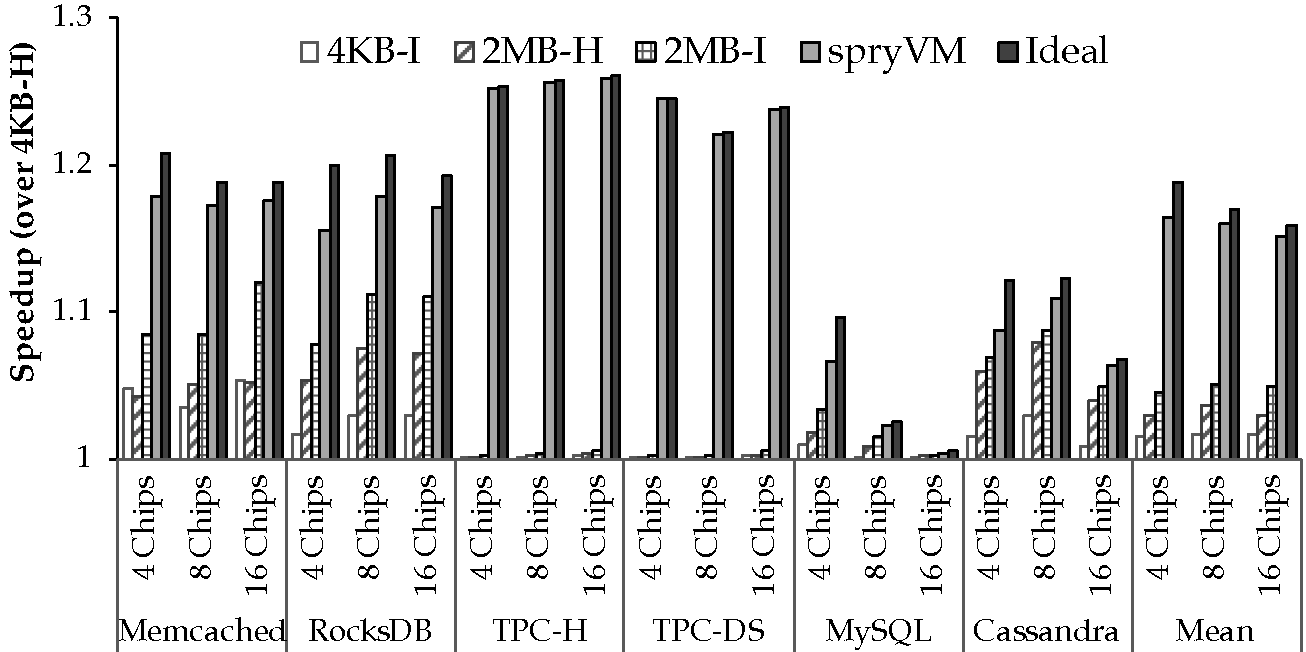
\includegraphics[width=0.48\textwidth,clip]{graphs/speedup_inmemory.pdf}
%   }
%
%
%  \subfloat[Out-of-memory scenario.]{
%  \label{fig:speedup_memory_out}
%
% 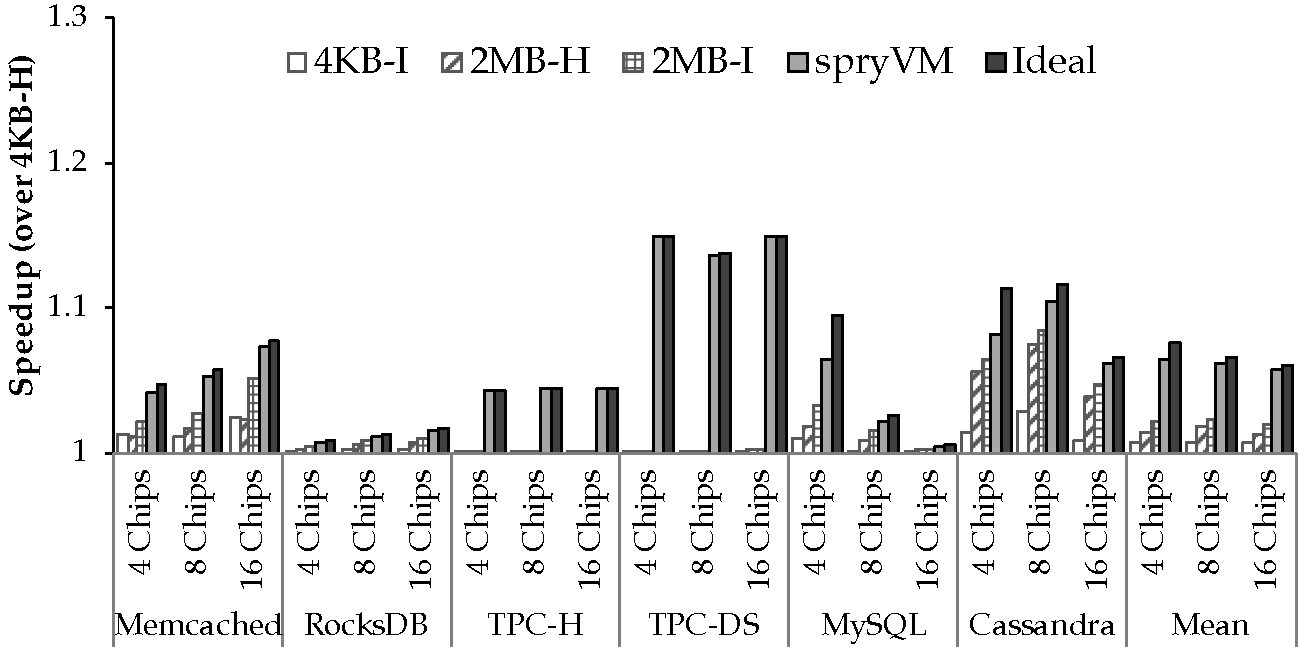
\includegraphics[width=0.48\textwidth,clip]{graphs/speedup_disk.pdf}
%  }



%\caption{Speedup over 4KB-H for 4KB-I, 2MB-H, 2MB-I, DTRIM, and an ideal translation.}
%  \label{fig:speedup_memory}
 
%\end{figure*}

%In this section, we perform a quantitative and qualitative study of the performance of different translation mechanisms.

We now perform a quantitative and qualitative study on VM.

\subsection{Performance Analysis}

The paper discusses many different workload scenarios and system configurations. As there are way too many performance points, we will show only the scenarios that have significant performance differences. First, we will show two workload scenarios, in-memory, where the memory size is equal to the working set size (i.e., the 1x ratio), and out-of-memory, where the working set size is eight times larger than the memory size (i.e., the 1/8x ratio). Second, as the performance across different process counts does not vary significantly, we are showing the average across runs. Third, the two topologies, daisy chain and mesh, behave similarly in terms performance, and hence we also present the average of both. Last, we present the results for different memory chip counts.

Fig.~\ref{fig:speedup_memory_in} shows the speedup of five translation mechanisms over the conventional MMU using 4KB pages and the hierarchical page table, labeled 4KB-H, for the in-memory scenario. The techniques are the conventional MMU using 4KB pages and the inverted page table, 2MB pages using the hierarchical and inverted page tables, DTRIM, and an ideal translation mechanism with zero translation overhead. We label the techniques as 4KB-I, 2MB-H, 2MB-I, DTRIM, and Ideal respectively. In the interest of space, we omit the results with 1GB pages, which perform better than 4KB pages but always worse than 2MB pages. The reason is that the number of entries in the MMU for 1GB pages is significantly limited, and server workloads have a large number of virtual segments which are accessed concurrently. First, we see that DTRIM clearly outperforms 4KB-H, 4KB-I, 2MB-H, and 2MB-I. In some cases by a large margin, up to $25\%$ for TPC-H. In other cases more moderately, $2.1\%$, $2\%$, $1.3\%$, and $0.5\%$ over 4KB-H, 4KB-I, 2MB-H, and 2MB-I respectively for MySQL. Most importantly, DTRIM is consistently on par with the ideal translation that incurs zero overhead for translation. Overall, DTRIM improves performance by $17.2\%$. $14\%$, $12.3\%$, and $10.5\%$ over 4KB-H, 4KB-I, 2MB-H, and 2MB-I respectively, and stays within 1.2\% of the ideal translation mechanism on average.

Fig.~\ref{fig:speedup_memory_out} presents the speedups for the out-of-memory scenario. As expected, the speedups are less significant that in the in-memory case. The reason is that all the cases incur the slowdown of resolving page faults, and therefore there are fewer accesses that can be accelerated. Still, DTRIM systematically performs better than the conventional MMU, $6.1\%$, $5.4\%$, $4.5\%$, and $4\%$ on average over 4KB-H, 4KB-I, 2MB-H, and 2MB-I respectively, and stays within 0.6\% of Ideal. 

Importantly, we model a greatly optimistic case when using $2$MB and $1$GB pages as we assume all pages are huge, with no generation overhead or fragmentation in any scenario. Additionally, we do not account for the excess in IO traffic generated by writing back dirty huge pages. Therefore, we expect further improvements with a realistic overhead. 

%Furthermore, we are conservatively assuming that all conflict page faults are major, and hence involve an access to secondary storage. Hence, in a real system, our speedups would likely be higher.


\subsection{Comparison with Other Proposals}

All the recent proposals on address translation for CPUs presented in Section~\ref{sec:uvm} aim to enhance the reach of TLBs by exploiting the contiguity available in the virtual and physical address spaces. Hence, these techniques are orthogonal to DTRIM as we reduce the TLB miss penalty. 

However, these techniques would be only effective for in-memory scenarios, and perform poorly for larger-than-memory working sets. In out-of-memory scenarios, direct segments~\cite{basu:efficient} would not be able to allocate the most frequently used pages in memory. Similarly, Redundant Memory Mappings and Hybrid TLB Coalescing~\cite{karakostas:redundant, park:hybrid} would not be able to allocate contiguous chunks of physical memory and fall back to base pages. CoLT~\cite{pham:colt} and Clustered TLBs ~\cite{pham:increasing} would also perform similar to the conventional translation when there is limited physical contiguity available. 

Even for in-memory scenarios, large address translation contiguity, on which proposed
TLB coalescing techniques rely~\cite{haria:devirtualizing,karakostas:redundant,gantz:hybrid,pham:colt,pham:increasing}, diminishes as the system runs. We adapt a representative kernel modification (increasing the max order of the buddy allocator), which enables large contiguous memory allocation (up to 1GB), to demonstrate the impact of memory fragmentation from long-run systems. We run a simple program \textit{mem\_sweep}, which allocates 30GB memory and accesses throughout all of it, along with our benchmarks back-to-back in our experimental machine with 32GB memory and measure the number of 1GB contiguous memory regions created by the modified kernel. Our program is able to obtain 28 of 1GB contiguous memory regions right after our experimental machine boots. The number decreases substantially to 8 at second round of execution and goes down to 5 (18\% of the number of 1GB contiguous memory regions at fresh boot time) after another 4 rounds of execution. The results show that memory fragmentation can significantly deter the contiguous memory creation, especially when the system's memory is fully utilized.
